%%%%%%%%%%%%%%%%%%%%%%%%%%%%%%%%%%%%%%%%%%%%%%%%%%%%%%%%%%%%%%%%%%%%%%%%%%%%%%%%
%2345678901234567890123456789012345678901234567890123456789012345678901234567890
%        1         2         3         4         5         6         7         8
% THESIS CHAPTER


\chapter{Control Architecture: Methods \& Results}
\label{chap:method}
\ifpdf
    \graphicspath{{Method/Figures/PNG/}{Method/Figures/PDF/}{Method/Figures/}}
\else
    \graphicspath{{Method/Figures/EPS/}{Method/Figures/}}
\fi

In this chapter, experimental set-up is described, and results given and discussed. The architecture is tested on a well defined scenario.\\
It is made up of two I-AUV's \href{https://cirs.udg.edu/auvs-technology/auvs/girona-500-auv/}{Girona 500 AUV} underwater vehicles, each one equipped with a CSIP Robot arm5E (4 DOF arm with a parallel yaw gripper). The final goal is to successfully coordinate the robots in such a way that the peg, hold by both manipulators, is inserted correctly in the other piece, fixed in the environment. 

The chosen strategy divides the problem in two phases: Hole Detection and Insertion. In the first preliminary step are done to detect the hole. A third robot, not used for manipulation task, is in charge to exploit vision to estimate the pose of the hole. Detail about this are given in section \ref{chap:vision}.
The second phase explores the problems inherent to the interaction between the peg and the hole, and the communication between the carrying agents. This is described in this chapter.
                          
%todo descrivi la situa: due piu uno robot, il peg, hole nel ambiete. e metti foto per mostrare ste cose

%todo dire in sect 1 blabla... ecc

\section{Simulators}
\label{sec:simulators}
A bit effort has been spent to choice a suitable simulator for the case. At the end, \href{http://www.irs.uji.es/uwsim/}{UWSim} [\cite{uwsim}] was chosen. It is a simulator largely used for this kind of scenarios, which visualize a virtual underwater scene. It provides a different variety of useful sensors (e.g. the used force-torque sensor and the cameras), but also others can be added. It is fully integrate in ROS, which made it really easy to use. ROS is used as simulator interface: through ROS messages, we can send commands to the robots and we can receive information from the going on test. Contact physics is implemented integrating the physics engine \href{https://pybullet.org/wordpress/}{Bullet} with \href{http://www.openscenegraph.org/}{OSG} through \href{https://github.com/mccdo/osgbullet}{OSGBullet}. To further details about how the simulation is implemented, especially the contact physics part, please refers to the documentation of the cited software. The cons in using UWSim is that the simulations is fully kinematic, so no dynamics interaction ar present. This means, for example, that velocity sent to the robot are immediately accomplished, and that we can't simulate the real physics while grasping a real object. For the scope of this thesis, this lack is not important because dynamics is not considered. Furthermore, the only needed dynamic part, i.e. how the contact between the tool and the hole affect the whole manipulator chain, can be simulated at kinematic level thanks to the information provided by the force-torque sensor, as explained in section \ref{sec:forceConsideration}.\\
To fill the lack of dynamic of UWSim, a good alternative can be \href{https://github.com/freefloating-gazebo/freefloating_gazebo}{FreeFloatingGazebo} [\cite{freeFloatingGazebo}]. In truth, this simulator is a plug-in for Gazebo and UWSim; it integrates them in order to achieve both dynamic (thanks to Gazebo) and visually realistic I-AUV simulation (thanks to UWSim). The interface used to communicate with the simulation is the same of UWSim, so ROS and its messages, which make it easy as UWSim to use. \\
This plug-in has been taken into consideration for dynamic test, that are not evaluated due to the lack of time, but can be certainly used for further works.
\href{http://gazebosim.org/}{Gazebo} is a generic simulator widely used in all robotics fields. It is the de-facto simulator for ROS. Seen its purpose, it is not a ready-to use simulator for underwater environment, and can be only a starting point to build a software to simulate this particular scenario (as it is done by FreeFloatingGazebo).\\
Also other simulators, \href{http://www.coppeliarobotics.com/index.html}{V-REP} [\cite{vrep}] and \href{https://cyberbotics.com/}{Webots} [\cite{webots}] have been taken into consideration but discarded for same \enquote{not ready-to-use} reason like Gazebo.\\
An interesting simulator is \href{https://github.com/disaster-robotics-proalertas/usv_sim_lsa}{USV simulator} [\cite{usvsim}] which takes the best from UWSim, Gazebo and FreeFloatingGazebo to implement realistic simulation. This is a really recent and in development project, and however it is focused more on surface vessels dynamics.\\

More details and comparisons are available in \cite{simComparisonCook} and \cite{usvsim}, and a schematic recap taken from \cite{usvsim} is visible in fig. \ref{fig:simComparison}.
\begin{figure}[H]
	\centering
	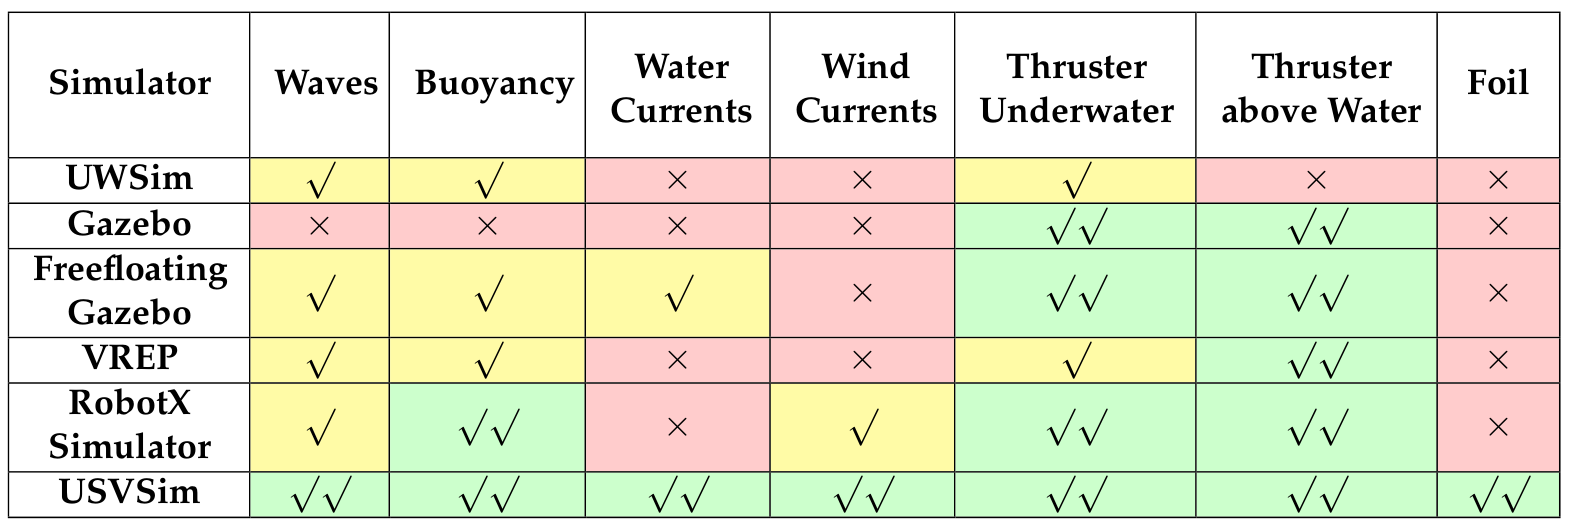
\includegraphics[width=14cm]{simComparison.png}
	\caption[Schematic Simulators Comparison]{Schematic recap of simulation comparison taken from \cite{usvsim}. $\times$ stands for no implemented feature; ~ $\surd\,$  for a feature that is a discrete representation of the real one; ~ $\surd\surd\,$ for a good representation of the real one. More details on how each feature is evaluated are available in the original paper.}
	\label{fig:simComparison}
\end{figure}

\section{Assumptions}
It is important to detail the main assumptions (related to the control architecture) made. A lot of problems, that it is necessary to take into account in a real environment, are not explored. This is necessary due to the difficulty of the particular scenario chosen.
\begin{itemize}
	\item Simulation is only kinematic. This implies, for example, that the commanded velocity to the vehicle and the arm are accomplished \textit{instantaneously} and \textit{perfectly}. Another implication is that the movements of arm and of the vehicle don't influence each other at all. The only \enquote{dynamic} implemented is caused by collision between the peg and the hole, which transfer the forces and torques acting on the peg along the whole arm. Disturbances of this type on the vehicle are neglected. (TODO %todo e invece ce le metterò?%)
	
	\item The initial configuration is with the peg already \textit{correctly} grasped by both robots. Also, the position of the grasped point and the peg dimension are known: this imply that relative position between robot and tip of the peg is \textit{perfectly} known. This initial condition is chosen because the grasping phase and problems arising during cooperative transportation have been explored in others cited project like MARIS and ROBUST (e.g in the work \cite{IntroMaris2}) and also as part of the on-going project TWINBOT.
	
	\item The peg is firmly grasped by both robot, no slippery is take into account. In truth, here an important detail must be explained. To the work purpose, and for simulator limitations, two pegs are modelled, each one like a fixed part of each robot. So it is truth that each peg is fixed respect to each agent, but the two pegs (perfectly overlapped at the beginning) can distance themselves. This is a useful benchmark to understand how good is the performance: the more the pegs distance themselves, the more we would apply a stress on the object (and on the arms) in a real situation.
	%todo vedi di riscrivere qua se usi la "colla" per tenere il secondo robot
	
	\item Pose (linear and angular displacement) of the two carrying robots and of the vision robot respect a common inertial frame is known. In real situation, knowing the position underwater is really an issue and it is never really precise. This information can be provided, for example, thanks to some mappings of the seafloor, to find a common interest point which refer to. Note that it is not important know the pose of the robot respect to a point above the water surface (that can be done thanks to information shared with surface vessels, for example as explored the WiMUST project [\cite{wimust}]). The important thing is to know relative pose of the robots to a common node, that can also be underwater. This is needed to make the vision robot share correctly the estimated pose of the hole.
	
	\item No real communication issues between the two carrying robot are taken into account. The presence of water put important issues in real situation; for example with water \textit{full-duplex} communication (i.e. sharing data \textit{at the same time}) is impossible, and in general a there is lower bandwidth than in the air. Some experiment in simulated environment with different methods of underwater communication are detailed in \cite{IntroMaris2}.\\
	The issues about communication are taken indirectly using a cooperative scheme (explained in section \ref{sec:coopScheme}) which permits to exchange few information between the two carrying agents.
	
	
	%todo altre? 
\end{itemize}

Others assumptions, more related to the vision part, are detailed in section \ref{sec:visioAssumption}.

\section{Tools}
The Control Architecture is implemented in C++ language, using various libraries. In this section, the most relevant libraries and tools used for the software are described. Please note that a particular section (section \ref{sec:simulators}) is dedicated to the chosen simulator UWSim.

\begin{itemize}
	\item \href{http://www.ros.org/}{\textbf{ROS}} (Robot Operating System), the well-known robotic middleware. It is used to communicate with the simulator, so to send commands to robots and receive information by the on-going simulations (e.g. robots states, information from sensors, streaming images from cameras).
	
	\item \href{http://eigen.tuxfamily.org/index.php?title=Main_Page}{\textbf{Eigen}} [\cite{eigen}], a C++ library for linear algebra. It is very useful to deal with matrices computations and management in any C++ software.
	
	\item \textbf{CMAT}, another C++ library, implemented at \href{http://www.graal.dibris.unige.it/}{GRAAL}. It implements the core functions for the TPIK method, detailed in \cite{IntroMaris1}.
	
	\item \href{http://www.orocos.org/kdl}{\textbf{Orocos KDL}} a package to deal with kinematic and dynamic chain. In the case of this thesis, it is used to compute the Jacobian of the robots for each of their configurations.
\end{itemize}


\section{qui spiega il task inseriti e in particular il force task}
%todo ricorda le force consideration della theory part

